% Template for ICASSP-2016 paper; to be used with:
%          spconf.sty  - ICASSP/ICIP LaTeX style file, and
%          IEEEbib.bst - IEEE bibliography style file.
% --------------------------------------------------------------------------
\documentclass{article}
\usepackage{spconf,amsmath,graphicx}
\usepackage{algpseudocode}
\usepackage{amssymb}
\usepackage{bm}

% Example definitions.
% --------------------
\def\x{{\mathbf x}}
\def\L{{\cal L}}

% Title.
% ------
\title{TOMOGRAPHIC RECONSTRUCTION FROM PROJECTIONS WITH UNKNOWN VIEW ANGLES EXPLOITING MOMENT-BASED RELATIONSHIPS}
%
% Single address.
% ---------------
\name{Eeshan Malhotra and Ajit Rajwade}
\address{Department of Computer Science and Engineering, IIT Bombay}
%
%
\begin{document}
%\ninept
%
\maketitle
%
\begin{abstract}
In this paper we describe a straightforward, yet effective method of recovering angles from a set of tomographic projections when the view-angles are completely unknown. Existing works on this problem have consistently assumed availability of projections from a large number of angles as well as made assumptions on the underlying distribution of angles to aid reconstruction. We make no such assumptions, and yet show a principled technique which is empirically validated, and quite robust to noise. 	
\end{abstract}
%
%\begin{keywords}
%computerized tomography, CT, angle recovery, unknown angles, image reconstruction, projections, projection moments, image moments
%\end{keywords}
%
\section{Introduction}
\label{sec:intro}
Commonly, in a parallel-beam tomographic formulation, the view angles are assumed to be perfectly known. However, there are many scenarios where this may not be the case. One such setting is cryo-electron microscopy (cryoEM), where tomographic techniques are used to determine the structure of a molecule or cell \cite{Frank1996}. Multiple repetitions of the procedure are performed on identical specimens, each of which is arbitrarily oriented. With no way to control the relative orientation of the replica specimens, the tomographic angles are essentially unknown. Another use case of such a technique is in insect tomography \cite{Walker2014}, or tomography of objects performing unknown rigid motion, which is equivalent to performing a tomographic reconstruction on a fixed object, with the view angles of the projects being unknown. Uncertainty in view angles, though to a lower degree, may also occur due to patient motion in medical imaging \cite{Wood1995}. 

In each of these scenarios, there may be significant or complete uncertainty in the angles from which tomographic projections are computed. It has been shown in \cite{uniqueness} that under certain modest conditions, the view angles can be uniquely determined from the tomographic projections, and that the estimated angles are in principle stable under noise \cite{feasibility} in almost all cases. However the associated algorithms rely on some strong assumptions. Most algorithms make use of the assumption that projections at nearby angles (or moments thereof) are similar to each other, and utilize this assumption to formulate an embedding of projections onto a lower-dimensional space using dimensionality reduction techniques. \cite{fangslle} uses Spherical Locally Linear Embedding (sLLE) to embed projections on a circular, 2-D space; \cite{fangmds} utilizes spherical multi-dimensional scaling to reduce dimensionality; \cite{graphlaplacian} uses a Laplacian graph-based manifold learning method to embed projections from various view angles on the circle. Others such as \cite{feasibility} have utilized simple heuristics like a nearest neighbour search to find angle ordering. In all cases, the essence of the methodology has been to find out an \textit{ordering} of angles. This suffers from multiple problems: First, since the assumptions are not mathematically driven, there is no theoretical guarantee on the resultant angles to satisfy the Helgasson-Ludwig Consistency conditions (See section \ref{ssec:descent}), which relate the geometric moments of the underlying image to those of its tomographic projections. Second, since the algorithms provide only an ordering on the angles, one must depend on knowledge of the \emph{underlying probability distribution} of the angles to recover the actual angle values. Lastly, the use of such methods necessitates the availability of projections from a large number of angles. Otherwise, the angle estimates have a large variance (Section III, \cite{graphlaplacian}). While in certain scenarios, obtaining a large number of measurements may be feasible, it is always advantageous to be able to reconstruct with a fewer view angles.
In this paper, we describe a method which is mathematically motivated, general in applicability, robust to a fair degree of noise, and viable even with projections from a few angles being available.
\section{BACKGROUND AND PROBLEM FORMULATION}
\label{sec:problem}
In the problem of (parallel beam) tomographic reconstruction, the input consists of a set of angles, $\bm\theta \triangleq \{ \theta_1, \theta_2, ..., \theta_P \}$ and the corresponding projections of a 2-D image from these angles, forming the set  $\bm{P_\theta} \triangleq \{ P_{\theta_i} \}_{i=1}^P$. A projection, $P_{\theta_i}$, is essentially a vector of line integrals of the image, as viewed from angle $\theta_i$ (from a fixed $0$ angle). That is, the $s^{th}$ element of the vector $P_{\theta_i}$, $P_{\theta_i}(s)$, is the line integral along a ray at a distance $s$ from the origin, and inclined at an angle $\theta_i$ to the y-axis. It is well known that given infinitely many such projections with known corresponding angles, the image can be reconstructed perfectly. However this is infeasible in practice. Hence, multiple techniques have been developed to reconstruct images from a sparse set of projections, \textit{e.g.}, the well-known filtered back-projection technique \cite{dipbook}, or moment-based methods such as \cite{imagemomentmethod}.

\subsection{Unknown View Angles}
In some applications, the exact angles in $\bm \theta$ are not known with precision, or not known at all. In such situations, there is an inherent ambiguity associated with the angles being recovered. Rotating the initial image by a fixed angle $\phi$ would produce the exact same set of projections, but at an angular shift of $\phi$. Further, reflecting the original image also allows for the same set of projections to be produced. Therefore, all angles will be determined with this inherent ambiguity. That is, we may have an inherent ambiguity as
$\hat{\theta_i} = \sigma\theta_i + 2n_i\pi + \phi$, where $\theta_i$ is the original angle from where the $i^\textrm{th}$ projection has been acquired, $\hat{\theta_i}$ is the estimated value of this angle, $\sigma \in \{+1,-1\}$, $n_i \in \mathbb{Z}$, and $\phi$ is the fixed rotational ambiguity. This is not a limitation as such, and we will evaluate the correctness of results allowing for such an ambiguity. It has been shown that provided a surprisingly small number of such projections, this problem permits a unique solution (allowing for aforementioned ambiguity) under very mild assumptions on the underlying image \cite{uniqueness}. Further, the same authors have also proved that such a solution is stable under noise in \cite{feasibility}. However, a constructive algorithm to illustrate this, which does not rely on stronger assumptions on the distribution of the angles, has not been published. In the following section, we describe an algorithm that empirically satisfies these criteria.

\section{ALGORITHM DESCRIPTION}
\label{sec:algo}
The complete process consists of three stages: (a) Denoising noisy tomographic projections, (b) Angle estimation through iterative coordinate descent, and (c) Image reconstruction using the estimated angles. In this work we provide algorithms for steps 1 and 2. Existing algorithms for step 3 perform quite well. For assessing the technique, we use the error in estimation of angles as a metric for evaluation. For testing, we have used filtered back-projection (FBP) algorithm for reconstruction for simplicity, though better algorithms inspired from the compressed sensing literature may be used \cite{kim2008interior}. 

\subsection{Denoising}
\label{ssec:denoising}
We used a patch-based PCA denoising method to reduce the noise in the projections. This algorithm is adapted from a similar algorithm for 2-D images, as described in \cite{Muresan03} (a popular method, widely used for denoising). We consider patches of size $d \times 1$ from a moving window across each projection. For each patch, we find its $L$ nearest patches (in the $L^2$-norm sense). We perform PCA on this set of $L$ vectors and project each one along the principal directions to produce eigencoefficients. To denoise the patch, we manipulate these coefficients using Wiener-like updates of the form $\hat{x_{il}} = y_{il} \bigg(\dfrac{\sigma_l^2}{\sigma_l^2 + \sigma^2}\bigg)$, where $\hat{x_{il}}$ is an estimate of the $l^{\textrm{th}}$ denoised coefficient for patch $i$ ($1 \leq l \leq d$), $y_{il}$ is the corresponding noisy coefficient for patch $i$, and $\sigma_l^2$ (the mean squared value of the $l^{\textrm{th}}$ coefficient across all $L$ patches) is estimated as: $\hat{\sigma_l^2} = \textrm{max}\bigg(0,\frac{1}{L}\sum\limits_{i=1}^L  {y_i^2 - \sigma^2}\bigg)$. 

Note that this is different from a PCA-based denoising approach as used in \cite{singer2013}, where entire projections are compared. The patch-based approach proposed above has two distinct advantages: (a) The use of patches (with size appropriately tuned) allows for similarity among different parts of the same projection as well; and (b) This method works even when the total number of projections is considerably lower. When finding similarity between entire projections in a small set, it is unlikely that we find very similar projections.

\subsection{Coordinate Descent}
\label{ssec:descent}
This is the key part of the algorithm. We utilize the Helgasson-Ludwig Consistency Conditions (HLCC) \cite{Natterer1986}, which describe the relationship between the geometric moments of the underlying image $f(x,y)$ and its projections from a given angle. For a particular angle $\theta_i$, the $n^{\textrm{th}}$ order moment of $P_{\theta_i}$ is calculated as follows:
\begin{equation}\label{PM}
m^{(n)}_{\theta_i} = \int_{-\infty}^{\infty} P_{\theta_i}(s) s^n ds
\end{equation}
Now, there exist $n+1$ image moments of the $n^{\textrm{th}}$ order. For natural numbers $p$, $q$, such that $p + q = n$, the $n^{\textrm{th}}$ order image moments can be calculated as \cite{dipbook}:
\begin{equation}
\upsilon_{p,q} = \int_{-\infty}^{\infty} \int_{-\infty}^{\infty} f(x,y) x^py^q dx dy
\end{equation}
The HLCC describe a relationship between the $n^{th}$ order projection moments and the $n^{\textrm{th}}$ order image moments: 
\begin{equation}\label{hlcc1}
m^{(n)}_{\theta_i} = \sum\limits_{j=0}^n  {n \choose j} (\cos{\theta_i})^{n-j}(\sin{\theta_i})^j \upsilon_{n-j,j}
\end{equation}
Using projection moments from multiple angles, (\ref{hlcc1}) can be written in matrix form, $\mathbf{m^{(n)}} = \mathbf{A^{(n)}} \boldsymbol{\upsilon^{(n)}}$
where, for the $n^{th}$ order equation, $\mathbf{A^{(n)}}$ is the $P \times (n+1)$ matrix defined by $\mathbf{A^{(n)}}_{ij} = {n \choose j} (\cos{\theta_i})^{n-j}(\sin{\theta_i})^j$, and $\boldsymbol{\upsilon^{(n)}} \triangleq \{\upsilon_{p,q} | p + q = n, p, q \in \mathbb{Z} \}$, and $\mathbf{m^{(n)}}$ is a vector containing the projection moments of order $n$ at $P$ different angles. This equation can be used to determine $\boldsymbol{\upsilon^{(n)}}$, and for this, we need $P \geq n+1$.

Since, in practice, the projections are noisy, despite denoising, equation \ref{hlcc1} will not be satisfied exactly. Further, uncertainty in the value of $\theta_i$s will translate into more approximation errors. In our problem setting, we do not actually know the values of $\theta_i$. We will, instead, use \textit{hypothesized} values of $\theta_i$. For hypothesized values of $\bm{\theta}$ and the set of image moments, $\bm{\upsilon} = \{\bm{\upsilon^{(n)}}\}_{n=0}^k$, we can define our energy function, $E$ as:
\begin{equation}\label{Ehlcc}
E(\bm{\theta}, \bm{\upsilon}) = \sum\limits_{n=0}^k \sum\limits_{i=1}^p \bigg(m^{(n)}_{\theta_i} - \sum\limits_{j=0}^n  \mathbf{A^{(n)}}_{i,j} \mathbf{\upsilon}_{n-j,j}\bigg )^2
\end{equation}
This equation is the crux of the algorithm. $E(\bm{\theta}, \bm{\upsilon})$ is the objective we must minimize by appropriately selecting values of the parameters $\bm{\theta}$ and $\bm{\upsilon}$. This is achieved through an iterative approach, where estimates for each $\theta_i$ are improved one at a time, and the values of $\bm{\upsilon}$ recalculated using a pseudo-inverse. We can now describe the iterative algorithm using coordinate descent.  
%\noindent\fbox{%
%\begin{minipage}{\dimexpr\linewidth-2\fboxsep-2\fboxrule\relax}%{1.8\columnwidth}
\begin{algorithmic}[1]
\State Randomly initialize $\bm{\theta}$ estimates, by picking each $\theta_i$ uniformly from $-\pi$ to $\pi$
\State Calculate projection moments, $\bm{m^{(j)}_{\theta_i}}$, of the first $1 \leq j \leq k$ orders.
\State Estimate image moments of the first $k$ orders, $\bm{\upsilon^{(i)}}$, $1 \leq i \leq k$. We only need $k+1$ view angles for this, but we set $k$ to a much lower value than the number of available views, to introduce redundancy into the system.
\State Calculate $E$ using \ref{Ehlcc}.
\State Set $\Delta E = \infty$
\While{$\Delta E > \epsilon$}
    \For{each $\theta_i$}
        \For{each angle in $-\pi$ to $\pi$, with appropriate resolution}
            \State Assume this value for $\theta_i$
            \State Recalculate image moments using this value
            \State Calculate $E$ again, using updated values of $\theta_i$ and image moments
            \If {$E$ $<$ previous-best-estimate}
                \State update the best estimate for $\theta_i$
                \State $\Delta E = $ Old value of $E$ $-$ new value of $E$
                \State Update the value of $E$
            \EndIf
        \EndFor
    \EndFor
\EndWhile
\end{algorithmic}
For each $\theta_i$, the algorithm performs a 1-D brute-force search for the value that minimizes $E$. The image moments are then re-estimated, and the value of $E$ updated
At each step, exactly one $\theta_i$ is updated. Since each update always reduces $E$, and $E$ is a non-negative quantity, it is guaranteed to converge eventually. In practice, it is seen that it takes a small number of iterations to converge. Further, the highest order moment to consider, $k$ is a tunable parameter. When we increase $k$ by $1$, we increase the number of knowns by $p$ - one known projection moment of order $k$ for each of the $p$ angles - and the unknowns by only $k$ - image moments of the $k^\textrm{th}$ order, introducing more redundancy in the system. So, in theory, it is feasible to use a very large $k$. However, in experiments, it was seen that while angle recovery generally improves with increasing the value of $k$, going beyond order 6 or 7, the gain was not noticeable, but increased computation time significantly.

The search space is not convex, and so, the convergence point using coordinate descent may be sensitive to initialization values of $\theta_i$s. To counteract this to a certain extent, we used a multi-start strategy, where the above algorithm is run multiple times, each time with a random initialization for $\bm\theta$. Finally, the iteration with the least value of $E$ at convergence is chosen as the optimal set of assignments for $\bm{\theta}$. Using this multi-start strategy, we almost always obtained accurate angle estimates.

\section{EXPERIMENTAL RESULTS}
\label{sec:results}
Experiments were conducted for multiple square images, with a size of 200x200 pixels, under zero mean, i.i.d. Gaussian noise with standard deviation varying from 1\% to 10\% of the standard deviation of the tomographic projections. It was observed that the final angles recovered were consistently close (almost entirely within $\pm 1^{\circ}$, occasional outliers reaching $\pm 5^{\circ}$) to the actual angles used to compute the projections. In each case, ten uniformly random initialization values were used for angle estimates, and the search was performed in $1^{\circ}$ steps. To test the robustness of the algorithm to different angle distributions, experiments were conducted on angles sampled from (a) a $(0,180) $ uniform distribution, (b) a non-uniform distribution, picking angles from each successive $30^{\circ}$ interval in the ratio 0.2:0.3:0.12:0.3:0.35 and (c) an extremely peaky distribution with 10 angle values sampled close to each of 10 randomly chosen, spread out peaks. We emphasize that knowledge of this distribution of the angles was \emph{not} used anywhere in our estimation algorithm. 

Reconstruction results using filtered back-projection and with a set of 30 angles as input for a particular image are included in Figure \ref{fig:recon} along with the angle estimation results in the top row of Figure \ref{fig:graphs}. Although, reconstructed images are also shown for visual interpretation, it should be noted that the reconstruction suffers from significant noise because of the limitations of FBP, and should be considered only in comparison to the baseline provided alongside. The quality of angle recovery can be seen in Figure \ref{fig:graphs} for different images and angle distributions at a noise level of 10\%.   

\subsection{Comparison with Existing Techniques}
We compared our results to the algorithm in \cite{singer2013} which in turn builds upon prior work in \cite{graphlaplacian} using the code provided by the authors. A further comparison was made with the  algorithm closely matching the one described in \cite{feasibility}.  These methods are representative of the class of methods that assume knowledge of the angle distribution. 

While both methods (\cite{feasibility, singer2013}) are indeed quite effective when the input consists of a large number of angles from a uniform distribution (even at incredibly low SNR), we observed in our experiments that they both fail completely (error greater than $30^{\circ}$) if either the number of angles is small (\textit{e.g.}, 30, as in the experiment here), or if the distribution is not uniform. The former result can be predicted directly from the variance of the angle estimates as evaluated in \cite{graphlaplacian}. 


\begin{figure}[htb]
\centering

\includegraphics[width=0.25\linewidth]{images/mickey_grey.jpg}
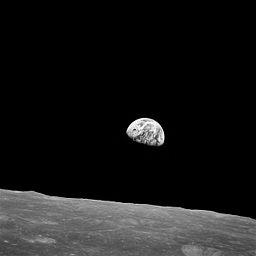
\includegraphics[width=0.25\linewidth]{images/earthrise_actual.jpg}
\caption{Original images used. Reconstruction results in Fig \ref{fig:recon}}
\label{fig:original}
\end{figure}


\begin{figure}[!ht]
%actual-5% {m30, m100, e100}
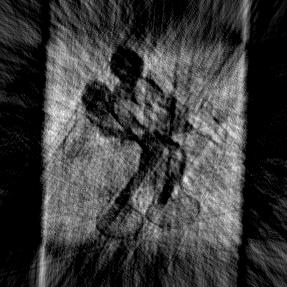
\includegraphics[width=0.3\linewidth]{images/mickey_nonunif_5pc_30_10_6_5_actualangles.jpg}
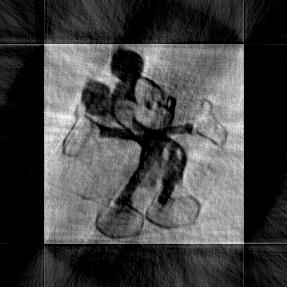
\includegraphics[width=0.3\linewidth]{images/mickey_nonunif_5pc_100_10_6_5_actualangles.jpg}
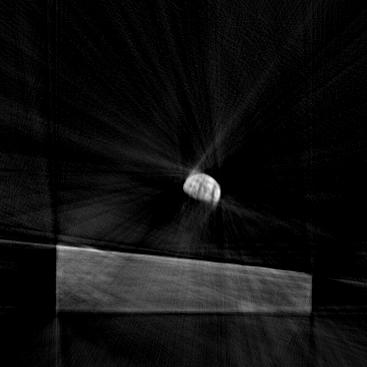
\includegraphics[width=0.3\linewidth]{images/earthrise_nonunif_5pc_100_10_6_5_actualangles.jpg}


%estimate-5% {m30, m100, e100}
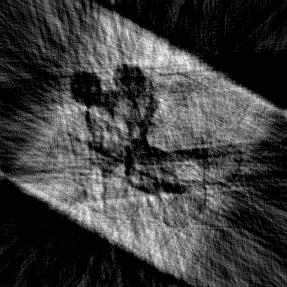
\includegraphics[width=0.3\linewidth]{images/mickey_nonunif_5pc_30_10_6_5_estimatedangles.jpg}
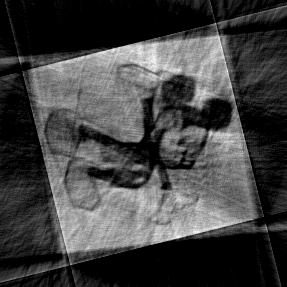
\includegraphics[width=0.3\linewidth]{images/mickey_nonunif_5pc_100_10_6_5_estimatedangles.jpg}
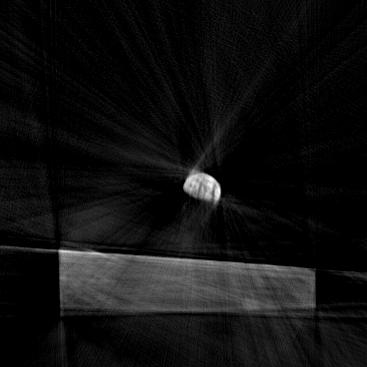
\includegraphics[width=0.3\linewidth]{images/earthrise_nonunif_5pc_100_10_6_5_estimatedangles.jpg}


%actual-10% {m30, m100, e100}
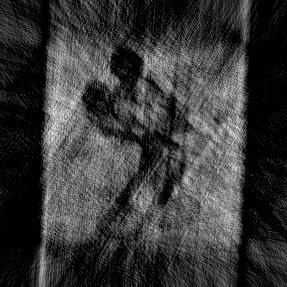
\includegraphics[width=0.3\linewidth]{images/mickey_nonunif_10pc_30_10_6_5_actualangles.jpg}
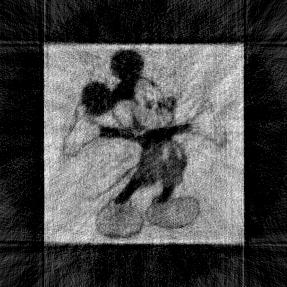
\includegraphics[width=0.3\linewidth]{images/mickey_nonunif_10pc_100_10_6_5_actualangles.jpg}
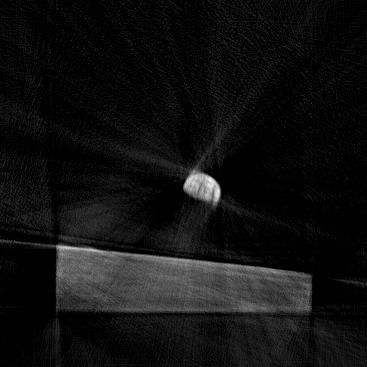
\includegraphics[width=0.3\linewidth]{images/earthrise_nonunif_10pc_100_10_6_5_actualangles.jpg}


%estimate-10% {m30, m100, e100}
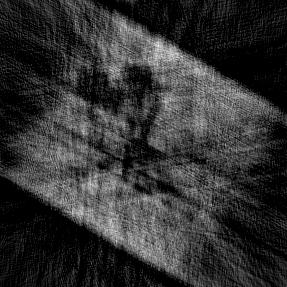
\includegraphics[width=0.3\linewidth]{images/mickey_nonunif_10pc_30_10_6_5_estimatedangles.jpg}
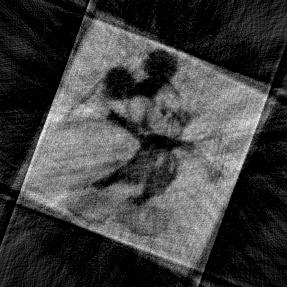
\includegraphics[width=0.3\linewidth]{images/mickey_nonunif_10pc_100_10_6_5_estimatedangles.jpg}
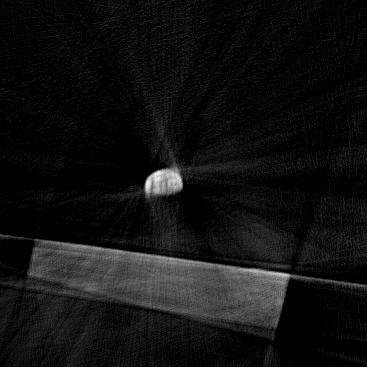
\includegraphics[width=0.3\linewidth]{images/earthrise_nonunif_10pc_100_10_6_5_estimatedangles.jpg}
\caption{FBP reconstruction using a non-uniform distribution of angles.
Top to bottom: Using (a) 5\% noise \& actual angles, (b) 5\% noise \& estimated angles, (c) 10\% noise \& actual angles (d) 10\% noise \& estimated angles
Reconstructions done with 30 angles (first column), 100 angles (second column), 100 angles (third column). 
Image canvas sizes have been expanded to allow for images to fit rotated reconstructions}
\label{fig:recon}
\end{figure}


\begin{table}[h!]
\centering
\caption{Statistics of errors in angle recovery, 5\% noise}
\label{angle-errors-table}
\begin{tabular}{|r|r|r|r|r|}
\hline
\textbf{Error} & \multicolumn{1}{c|}{\textbf{\begin{tabular}[c]{@{}c@{}}Earthrise\\ 30 angles\end{tabular}}} & \multicolumn{1}{c|}{\textbf{\begin{tabular}[c]{@{}c@{}}Earthrise\\ 100 angles\end{tabular}}} &
\multicolumn{1}{c|}{\textbf{\begin{tabular}[c]{@{}c@{}}Mickey\\ 30 angles\end{tabular}}} & \multicolumn{1}{c|}{\textbf{\begin{tabular}[c]{@{}c@{}}Mickey\\  100 angles\end{tabular}}} \\ \hline
$\leq 1^{\circ}$ & 13 & 94 & 20 & 66 \\
$\leq 3^{\circ}$ & 29 & 99 & 29 & 96 \\
$\leq 5^{\circ}$ & 30 & 100 & 29 & 100 \\
$> 5^{\circ}$ & 0 & 0 & 1 & 0\\ \hline
\end{tabular}
\end{table}


\begin{figure}[htb]
\centering
  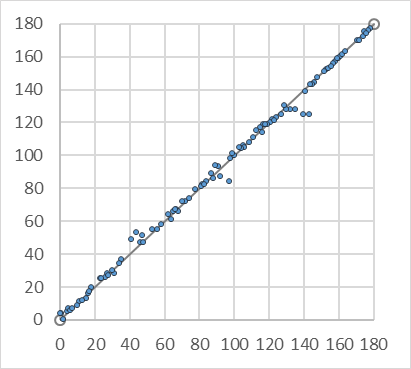
\includegraphics[width=0.4\linewidth]{images/graphs/m-unif-10pc-100.png}
  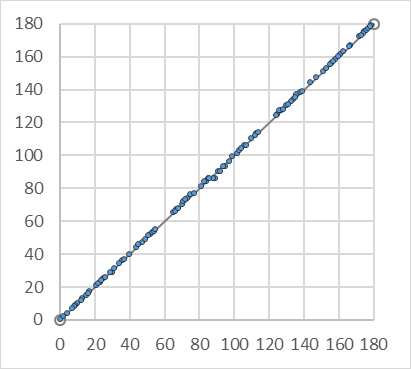
\includegraphics[width=0.4\linewidth]{images/graphs/e-unif-10pc-100.png}

  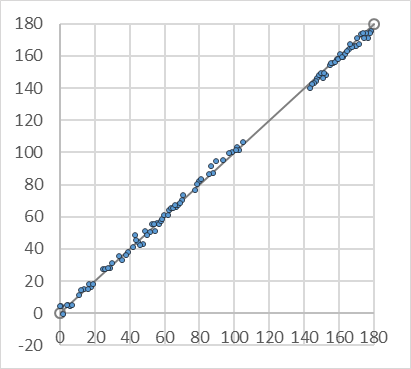
\includegraphics[width=0.4\linewidth]{images/graphs/m-nonunif-10pc-100.png}
  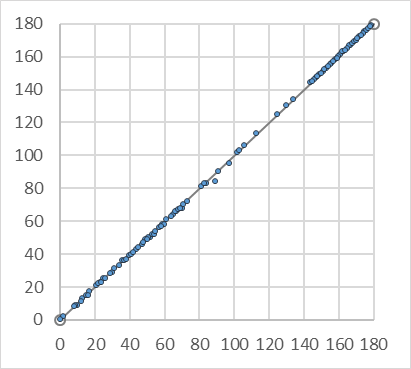
\includegraphics[width=0.4\linewidth]{images/graphs/e-nonunif-10pc-100.png}
  
  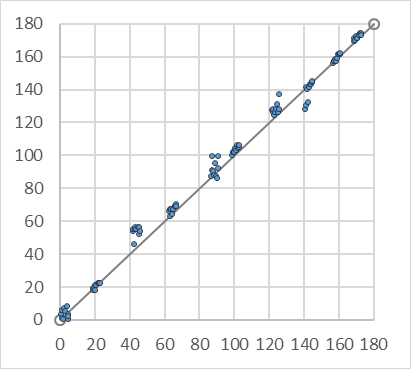
\includegraphics[width=0.4\linewidth]{images/graphs/m-peaky-10pc-100.png}
  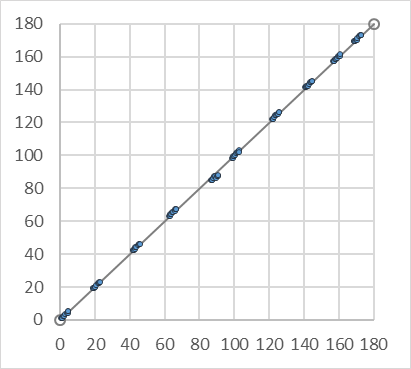
\includegraphics[width=0.4\linewidth]{images/graphs/e-peaky-10pc-100.png}
  
  
\caption{In each figure, X and Y axes show true and estimated angles respectively, under 10\% noise. Left: image `mickey'; Right: image `earthrise'.
Angles drawn from - Top row: a uniform distribution; Middle: a non-uniform distribution; Bottom: very peaky distribution.
For visualization, the offset $\phi$ in the estimated angles has been removed manually}
\label{fig:graphs}
\end{figure}

\section{SUMMARY AND CONCLUSIONS}
\label{sec:conclusions}
We proposed a general method for image reconstruction from projections from unknown view angles and empirically demonstrated its efficiency in a wide variety of scenarios - with varying number of view angles, with different distributions for generation of the angles, and at multiple noise levels. The key idea is to iteratively improve angle estimates to reduce HLCC residuals, using a coordinate descent strategy.

On experimenting with values of the maximum order of image moments to be considered, it was discovered that there is a clear trade-off between accuracy and computational time, but only up to a (fairly low) threshold, after which, increasing the order causes no noticeable improvement in the recovered angles. However, this remains a parameter which must be tuned by the user. In practical applications, besides unknown view angles, different projections could be acquired at different and unknown shifts. This scenario can be handled easily assuming the background intensity as 0, since that would produce projections padded with an appropriate number of zeros.   

There exist several open avenues for future research, such as handling projections with impulse noise or missing bins, projections with fan-beam geometry, reconstructions of 3D objects, and exploring the relationship of this problem with tasks such as automated instrument calibration in compressed sensing.


\vfill\pagebreak

\bibliographystyle{IEEEbib}
\bibliography{references}

\end{document}